\documentclass{article}[18pt]
\usepackage{../../../../../format}
\lhead{CSys - Databases}


\begin{document}
\begin{center}
\underline{\huge Relational Calculus and Relational Algebra}
\end{center}
\section{Relational Calculus and Algebra}
\textbf{Relational Calculus}: Formal definition of a new relation from existing relations in the DB\\
\textbf{Relational Algebra}: How to build a new relation from existing relations in the DB\\
\\
Their place in the big picture
\begin{center}
	\includegraphics[scale=0.7]{"big picture"}
\end{center}
\begin{itemize}
	\item Relational calculus
	\begin{itemize}
		\item Relations are considered as \textbf{sets of elements} (attribute values)
		\item The new relation is defined from the old one(s) using a set theoretic expression
	\end{itemize}
	\item Relational algebra
	\begin{itemize}
		\item Based on mathematical relations (tables)
		\item A theoretical language with operations on one (or more) input relations (tables) to define one new (output) relation
		\item The input relation(s) remain unchanged
	\end{itemize}
	\item Relational Algebra and Calculus
	\begin{itemize}
		\item Based on logic; equivalent languages (same expressive power)
		\item For every algebra expression $\leftrightarrow$ an equivalent calculus expression
	\end{itemize}
	\item Both are formal and non user friendly languages
	\begin{itemize}
		\item Used as the basis for higher level DML such as SQL
	\end{itemize}
	\item A query language is \textbf{relationally complete} if it can be used to produce any relation that can be derived using relational algebra/calculus expressions
	\item Most modern query languages (like SQL)
	\begin{itemize}
		\item Are relationally complete
		\item Have additional operations (summing, grouping, ordering)
		\item More expressive power than relational algebra
		\item But still not expected to be "Turing complete"
	\end{itemize}
\end{itemize}
\section{Relational Calculus}
In first order logic (or 'predicate calculus'):
\begin{itemize}
	\item Predicate: Truth valued function (true/false) with arguments
	\item Proposition: The expression obtained when we substitute values to the arguments of a predicate (can be true/false)
	\item Let $P(x)$ and $Q(x)$ be two predicates with argument $x$. Then:
	\begin{itemize}
		\item The 'set of all $x$ such that both $P(x)$ and $Q(x)$ are true' is:
		$$\{x|P(x)\land Q(x)\}$$
		\item The 'set of all $x$ such that $P(x)$ or $Q(x)$ is true' is:
		$$\{x|P(x)\lor Q(x)\}$$
		\item The 'set of all $x$ such that $P(x)$ is not true' is:
		$$\{x|\sim P(x)\}$$ 
	\end{itemize}
\end{itemize}
\section{Tuple Relational Calculus}
\begin{itemize}
	\item Variables $\leftrightarrow$ Tuples of a relation
	\item Aim: To find tuples for which some predicate(s) is true
	\item To specify that a tuple S belongs to the relation \texttt{Staff} we use the predicate \texttt{Staff(S)}
	\item Examples
	\begin{itemize}
		\item All tuples S of the relation \texttt{Staff} that have salary $>10000$
		$$\{S|Staff(S)\land S.salary>10000\}$$
		\item The salaries of all members of staff which earn $>10000$
		$$\{S.salary|Staff(S)\land S.salary>10000\}$$
	\end{itemize}
\end{itemize}
Domain relational calculus (another type of calculus):
\begin{itemize}
	\item Variables take values from domains of attributes of a relation (instead of tuples)
\end{itemize}
\begin{itemize}
	\item Use of quantifiers while building predicates:
	\begin{itemize}
		\item Existential quantifier $\exists$ (there exists)
		\item Universal quantifier $\forall$ (for all)
	\end{itemize}
	\item Tuple variables that are:
	\begin{itemize}
		\item Quantified by $\exists$ or $\forall$ $\rightarrow$ 'bound variables'
		\item Not quantified by $\exists$ or $\forall$ $\rightarrow$ 'Free variables'
	\end{itemize}
\end{itemize}
Example:\\
\textit{The names of all staff members who work in a branch in london}:
$$\{S.name|Staff(S)\land (\exists B)(Branch(B)\land (B.branchNo=S.branchNo)\land (B.city='London'))\}$$
Here S.name is a free variable and B is a bound variable
\section{Relational Algebra}
\begin{itemize}
	\item Both input and output are relations
	\begin{itemize}
		\item The output can become input to another relation
		\item Expressions can be nested
		\item This property is called "closure"
	\end{itemize}
	\item Relations are \textbf{closed} under Relational Algebra in the same sense as "numbers are closed under arithmetic expressions"
	\item In Relational Algebra all involved tuples from the input relation(s) are manipulated in one statement (with no loops)
\end{itemize}
\begin{itemize}
	\item Six basic operations in two categories:
	\begin{itemize}
		\item Unary operations
		\begin{itemize}
			\item Selection $(\sigma)$
			\item Projection $(\pi)$
			\item Rename $(\varrho)$
		\end{itemize}
		\item Binary operations
		\begin{itemize}
			\item Union ($\cup$)
			\item Set Difference $(-)$
			\item Cartesian Product $(\times)$
		\end{itemize}
	\end{itemize}
	\item Several derived operations (that can be expressed using the basic operations)
	\begin{itemize}
		\item Intersection $(\cap)$
		\item Division $(\div)$
		\item Join (Natural Join, Equi-Join, Theta Join, Outer Join, Semi-Join)
	\end{itemize}
\end{itemize}
\section{Selection}
$\sigma_{predicate}(R)$
\begin{itemize}
	\item Unary operation i.e. it works on a single relation R
	\item Outputs a subset of the relation R that contains only the tuples (rows) that satisfy the specified condition (predicate)
	\item i.e. it returns a "Horizontal Slice" of R
\end{itemize}
\section{Projection}
$\Pi_{\text{col-1,...,col-n}}(R)$
\begin{itemize}
	\item Unary operation
	\item Outputs a subset of the relation R that contains only the specified attributes (columns) with names $col-1,...,col-n$ and also eliminates duplicates
	\item i.e. it returns a "vertical slice" of R (by removing non-matching attributes)
	\item It can be combined with a selection
\end{itemize}
\section{Union}
$R\cup S$
\begin{itemize}
	\item Binary operation
	\item Outputs a new relation having all tuples of R, or S, or both R and S, and also eliminates duplicate tuples
\end{itemize}
That is:
\begin{itemize}
	\item It combines the rows from both tables, removing any redundant (common) row in the process
	\item If R has I tuples and S has J tuples, the output relation will have at most $I+J$ tuples
\end{itemize}
\section{Set Difference}
$R-S$
\begin{itemize}
	\item Binary operation
	\item Outputs a new relation having all tuples that exist in R but not in S
\end{itemize}
That is:
\begin{itemize}
	\item It removes from R any common rows that appear in both tables R and S
	\item If R has I tuples and S has J tuples, the output relation will have at least $I-J$ tuples
	\item Similarly, $S-R$ removes from S its common rows with R
\end{itemize}
\section{Union Compatibility}
To compute $R\cup S$ and $R-S$
\begin{itemize}
	\item The schemas of the relations R and S must match, i.e.:
	\begin{itemize}
		\item R and S must have the same number of attributes
		\item Every pair of corresponding attributes must have the same domain
	\end{itemize}
	\item The R and S are called union-compatible
\end{itemize}
If one of the relations has extra attributes the usual trick is to use projection to create union-compatible relations
\section{Intersection}
$R\cap S$
\begin{itemize}
	\item Binary operation
	\item The output relation has all tuples existing in both R and S
\end{itemize}
That is:
\begin{itemize}
	\item It removes from R any rows that appear only in R
	\item Equivalently: It removes from S any rows appearing only in S
	\item If R has I tuples and S has J tuples, the output relation will have at most $min\{I,J\}$ tuples
\end{itemize}
To compute $R\cap S$ the relations R and S must be union-compatible\\
\\
Intersection is a derived operation
$$R\cap S=R-(R-S)$$
\section{Cartesian Product}
$R\times S$
\begin{itemize}
	\item Binary operation
	\item Outputs a new relation that is a concatenation of every tuple from R with every tuple from S
	\item No further "compatibility" assumptions on the relations
	\item Recall: the ordering of the tuples does not matter
\end{itemize}
That is:
\begin{itemize}
	\item It "multiplies" the relations R and S
	\item If R has I tuples, N attributes and S has J tuples, M attributes then $R\times S$ has $(I*J)$ tuples and $(N+M)$ attributes
\end{itemize}
If R and S have attributes with the same name:
\begin{itemize}
	\item The attribute names are prefixed with the relation name
	\item e.g. $R.name$ and $S.name$
\end{itemize}
\section{Rename}
Relational Algebra operations can be very complex:
\begin{itemize}
	\item We decompose it into a series of smaller operations
	\item We give names to the intermediate operations (to reuse them)
	\item For this we iteratively use the assignment operation $"\leftarrow"$
\end{itemize}
A simple (but very useful alternative)
\begin{itemize}
	\item The rename operation $\varrho_X(E)$ returns E renames as X
	\item Moreover: $\varrho_{X(A_1,A_2,...,A_n)}(E)$ returns E renamed as X, where the attributes of X are defined as $A_1,A_2,...,A_n$
\end{itemize}
Especially useful when, for example:
\begin{itemize}
	\item We want to compute a join of a relation with itself (i.e. we can create a copy of the relation with a different name)
\end{itemize}
\section{Division}
$R\div S$
\begin{itemize}
	\item Binary operation, i.e. it works on two relations R and S
	\item A particular type of query that appears often in applications
\end{itemize}
Notation:
\begin{itemize}
	\item Let R have the set of attributes A
	\item Let S have the set of attributes B, where $B\subseteq A$
	\item Define $C=A-b$ (i.e. the attributes of R that are not in S)
\end{itemize}
The division operator $R\div S$ outputs a relation over the attributes C that consists of the tuples from R that match every tuple in S\\
\\
Division $R\div S$ is a derived operation
\begin{itemize}
	\item Compute all C-tuples of R that are not "disqualified" by a tuple in S
	\item A C-tuple of R is "disqualified", if by attaching it to a tuple of S, we obtain a tuple that is not in R
	\item Disqualified C-tuples of  R: $\Pi_C((\Pi_C(R)\times S)-R)$
	\item Tuples of $R\div S$: $\Pi_C(R)$- disqualified tuples
\end{itemize}
\section{Join}
\begin{itemize}
	\item The combination of Cartesian product and Selection can be reduced to a single operation, called a Join
	\item A Join is equivalent to:
	\begin{itemize}
		\item Build the Cartesian product of the two operand relations 
		\item Perform a Selection (using the join predicate F)
	\end{itemize}
	\item Notation
	\begin{itemize}
		\item $R\bowtie_F S=\sigma_F(R\times S)$ where F is a predicate
		\item If F contains only "=", then this is an Equijoin
	\end{itemize}
\end{itemize}
\section{Natural Join}
\begin{itemize}
	\item $A_1,A_2,...,A_k$: common attributes of relations R and S
	\item $R\bowtie S=\Pi_{C_1,...,C_x}(\sigma_{R.A_1=S.A_1,...,R.A_k=S.A_k}(R\times S))$\\
	Where $C_1,...,C_x$ are the attributes of $R\times S$ without the duplicates
	\item It is an equijoin of the relations R and S over all their attributes that have the same name, without duplications
\end{itemize}
Steps:
\begin{itemize}
	\item $R\times S$
	\item For each attribute with the same name A in both R and S, select the tuples where $R.A=S.A$ (from $R\times S$)
	\item Remove one of the duplicate columns corresponding to the above pairs of attributes
\end{itemize}
\section{Summary}
\begin{center}
	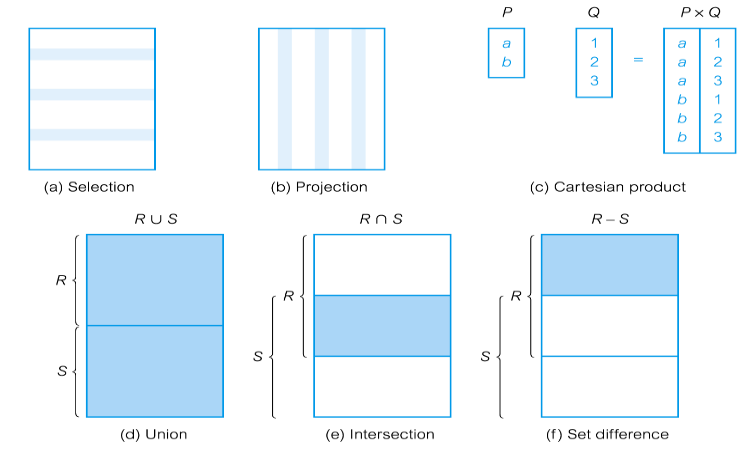
\includegraphics[scale=0.7]{Summary}
\end{center}

\end{document}